% Auto-generated answer document. Original problem statements are preserved verbatim.
\documentclass[11pt]{article}
\usepackage{fontspec}
\usepackage{microtype}
\usepackage{mathtools,amssymb,amsfonts,amsthm,bm}
\usepackage{enumitem}
\usepackage{geometry,fancyhdr,setspace,xcolor}
\usepackage{fancyvrb}
\usepackage{pdfpages}
\usepackage[hidelinks]{hyperref}
\geometry{margin=1in,headheight=14pt}
\setstretch{1.15}
\setlength{\parindent}{0pt}
\setlength{\parskip}{0.55em plus 0.12em minus 0.08em}
\setlength{\abovedisplayskip}{0.85em plus 0.2em minus 0.1em}
\setlength{\belowdisplayskip}{0.85em plus 0.2em minus 0.1em}
\setlist{leftmargin=*,topsep=0.35em,itemsep=0.15em,parsep=0pt}
\pagestyle{fancy}
\fancyhf{}
\fancyhead[L]{\coursename}
\fancyhead[C]{\assignment}
\fancyhead[R]{\studentname}
\fancyfoot[C]{\thepage}
\newcommand{\studentname}{Keshav Ramamurthy}
\newcommand{\coursename}{Math 110}
\newcommand{\assignment}{Homework 3}
\newcommand{\term}{Fall 2026}
\newcommand{\R}{\mathbb{R}}
\newcommand{\C}{\mathbb{C}}
\newcommand{\Q}{\mathbb{Q}}
\newcommand{\Z}{\mathbb{Z}}
\newcommand{\N}{\mathbb{N}}
\newcommand{\F}{\mathbb{F}}
\newcommand{\K}{\mathbb{K}}
\newcommand{\E}{\mathbb{E}}
\newcommand{\Prob}{\mathbb{P}}
\newcommand{\abs}[1]{\left\lvert#1\right\rvert}
\newcommand{\norm}[1]{\left\lVert#1\right\rVert}
\newcommand{\ip}[2]{\left\langle#1,#2\right\rangle}
\newcommand{\set}[1]{\left\{#1\right\}}
\newcommand{\given}{\,\middle\vert\,}
\newcommand{\dd}{\,\mathrm{d}}
\DeclareMathOperator{\rank}{rank}
\DeclareMathOperator{\nullity}{nullity}
\DeclareMathOperator{\Span}{span}
\DeclareMathOperator{\Ker}{ker}
\DeclareMathOperator{\im}{im}
\DeclareMathOperator{\Hom}{Hom}
\DeclareMathOperator{\Aut}{Aut}
\DeclareMathOperator{\Var}{Var}
\DeclareMathOperator{\Cov}{Cov}
\newtheorem{problem}{Problem}[section]
\newenvironment{solution}{%
  \par\smallskip\noindent\textbf{Solution notes}\par
  \vspace{1.15in}\noindent\hrulefill\par\vspace{0.28in}%
}{\par}
\newenvironment{originalproblem}{%
  \VerbatimEnvironment
  \par\medskip\noindent\begin{minipage}{0.98\linewidth}
  \begin{Verbatim}[fontsize=\small]%
}{%
  \end{Verbatim}\end{minipage}\par
}
\renewcommand{\coursename}{Math 110}
\renewcommand{\assignment}{Homework 3 Answers}
\begin{document}
\begin{center}\Large\textbf{Math 110 -- Homework 3 Answers}\end{center}
\includepdf[pages=3-4,pagecommand={\thispagestyle{empty}}]{hw_packet.pdf}
\clearpage
\section*{Solutions}
\subsubsection*{Problem 1}
\begin{solution}
% Write your proof, calculation, or argument here.
\end{solution}
\subsubsection*{Problem 2}
\begin{solution}
% Write your proof, calculation, or argument here.
\end{solution}
\subsubsection*{Problem 3}
\begin{solution}
% Write your proof, calculation, or argument here.
\end{solution}
\subsubsection*{Problem 4}
\begin{solution}
% Write your proof, calculation, or argument here.
\end{solution}
\subsubsection*{Problem 5}
\begin{solution}
% Write your proof, calculation, or argument here.
\end{solution}
\subsubsection*{Problem 6}
\begin{solution}
% Write your proof, calculation, or argument here.
\end{solution}
\subsubsection*{Problem 7}
\begin{solution}
% Write your proof, calculation, or argument here.
\end{solution}
\end{document}
